\documentclass[a4paper,11pt]{article}
\usepackage{a4wide}
\usepackage{fullpage}
\usepackage[toc,page]{appendix}
\usepackage[pdftex]{graphicx} % for figures
\usepackage{setspace}
\usepackage{color}
\definecolor{light-gray}{gray}{0.95}
\usepackage{listings} % for inclusion of Python code
\usepackage{hyperref}
\renewcommand{\baselinestretch}{1.2}

\lstset{ % style for Python code, improve if needed
language=Python,
basicstyle=\footnotesize,
basicstyle=\ttfamily\footnotesize\setstretch{1},
backgroundcolor=\color{light-gray},
}

\title{Mini Project \#1: Where are the Genes is due}
\author{Matjaž Mav (63130148)}
\date{\today}

\begin{document}

\maketitle

\section{Introduction}

In this assignment we had implement the gene-finding algorithm and then use it to analyze the genome of the \textit{Mycoplasma genitalium}.

\section{Implementation}
We analyzed all open reading frames, using slightly modified translation table 4. We used only one start codon \textit{ATG} and two stop codons \textit{TAA} and \textit{TAG}, since using full translation table resulted into much higher recall.

\section{Results}

\begin{enumerate}
    \item \textbf{What is the size of \textit{Mycoplasma genitalium} genome?}
    \\580076 bp
    \item \textbf{How many genes does it include?}
    \\509
    \item \textbf{What is the length of the smallest and the longest gene (in codons)? What is the median length of the gene (in codons)?}
    \\Shortest length: 38
    \\Longest length:  1806
    \\Median length:   288
    \item \textbf{What is the recall/precision of your gene finding procedure at L=50 and L=125 codons?}
    \\At length of 50 codons the precision is 0.12 and the recall 0.85.
    \\At length of 125 codons the precision is 0.20 and the recall 0.75.

    \begin{figure}[htbp]
    \begin{center}
    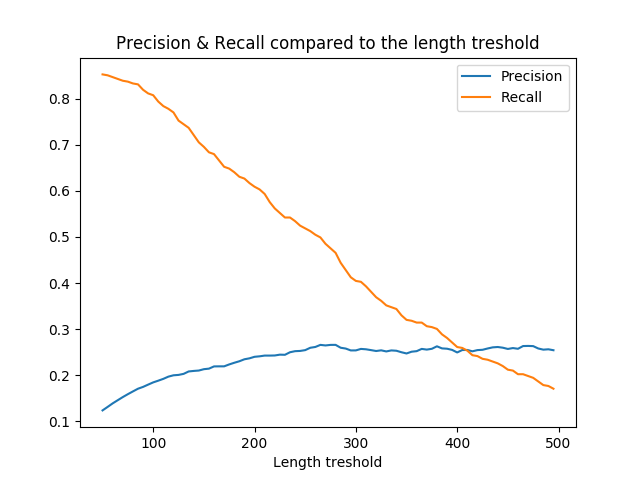
\includegraphics[scale=1.0]{plot.png}
    \caption{Comparison of the precision and recall to the length threshold}
    \label{fig-example}
    \end{center}
    \end{figure}
\end{enumerate}

\end{document}
